\documentclass[11pt,letterpaper]{article}
\usepackage[lmargin=1in,rmargin=1in,tmargin=1in,bmargin=1in]{geometry}
\usepackage{../style/homework}
\setbool{quotetype}{true} % True: Side; False: Under
\setbool{hideans}{false} % Student: True; Instructor: False

% -------------------
% Content
% -------------------
\begin{document}

\homework{20: Due 04/24}{Okay. No hard feelings, but I hate you. Not joking. Bye.}{Gina Linetti, Brooklyn 99}

% Problem 1
\problem{10} Consider the polynomial $f(x)= x^3 (x^2 + 1) (x + 4)^2 (x - 5) (x + 8)^3$. 
	\begin{enumerate}[(a)]
	\item What is the degree of $f(x)$?
	\item How many real zeros does $f(x)$ have?
	\item How many complex zeros does $f(x)$ have?
	\item Does $f(x)$ have a maximum or a minimum? Explain. 
	\end{enumerate} \pspace

\sol 
\begin{enumerate}[(a)]
\item The degree of $p_1(x) p_2(x) \cdots p_m(x)$, where the $p_i(x)$ are polynomials, are is the sum of the degrees of the $p_i(x)$. But then the degree of $f(x)$ is $3 + 2 + 2 + 1 + 3= 11$. \pspace

\item Setting $f(x)= 0$, we have $x^3 (x^2 + 1) (x + 4)^2 (x - 5) (x + 8)^3= 0$. This implies that either $x^3= 0$, which implies that $x= 0$ is a root with multiplicity 3, or $x^2 + 1= 0$, which implies $x^2= -1$ (not possible over the real numbers), or $(x + 4)^2= 0$, which implies that $x= -4$ is a root with multiplicity 2, or $x - 5= 0$, which implies $x= 5$ is a root with multiplicity 1, or $(x + 8)^3= 0$, which implies $x= -8$ is a root with multiplicity 3. Therefore, $f(x)$ has four distinct real zeros---or nine real roots when counting multiplicity. \pspace

\item From (b), we see the complex zeros of $f(x)$ `come from' the $x^2 + 1$ term. If $x^2 + 1= 0$, then $x^2= -1$. But then $x= \sqrt{-1}= \pm i= \pm i$. Therefore, $f(x)$ has two complex zeros. Alternatively, from the Fundamental Theorem of Algebra, we know that $f(x)$ must have 11 real or complex zeros (counting multiplicity). From (b), we know that nine of these roots are real. Therefore, $f(x)$ must have two complex zeros. \pspace

\item From (a), we know the degree of $f(x)$ is 11---which is odd. Therefore, the `ends' of $f(x)$ point in the opposite `direction.' But then $f(x)$ has neither a maximum nor a minimum value. 
\end{enumerate}



\newpage



% Problem 2
\problem{10} Determine the real quadratic polynomial that has a root at $x= 1 + 3i$ and has $y$-intercept 1. \pspace

\sol For a quadratic polynomial to be real, the complex roots must come in complex conjugate pairs. Therefore, if $1 + 3i$ is a root for the polynomial, $\overline{1 + 3i}= 1 - 3i$ must be a root of the polynomial. Because a quadratic polynomial has degree two (by definition), it must have exactly two roots (counting complex roots and counting roots with multiplicity) by the Fundamental Theorem of Algebra. Because we have two roots, namely $1 \pm 3i$, these must be all the roots of the polynomial. But then the polynomial must have the form\dots
	\[
	\begin{gathered}
	A \big(x - (1 + 3i) \big) \big(x - (1 - 3i) \big) \\[0.3cm]
	A (x^2 - x(1 - 3i) - x(1 + 3i) + (1 + 3i)(1 - 3i) \big) \\[0.3cm]
	A \big(x^2 - x + 3ix - x - 3ix + (1 - 3i + 3i - 9i^2) \big) \\[0.3cm]
	A \big(x^2 - 2x + 1 + 9(-1) \big) \\[0.3cm]
	A(x^2 - 2x + 10) 
	\end{gathered}
	\]  \pspace
We know this polynomial must have $y$-intercept of 1; that is, $y= 1$ when $x= 0$. But then\dots
	\[
	\begin{gathered}
	1= A(0^2 - 2(0) + 10) \\[0.3cm]
	1= 10A \\[0.3cm]
	A= \dfrac{1}{10}
	\end{gathered}
	\] \pspace
Therefore, it must be that the polynomial is\dots
	\[
	\dfrac{1}{10}\, (x^2 - 2x + 10)
	\]



\newpage



% Problem 3
\problem{10} Suppose that $f(x)$ is a degree five polynomial (quintic polynomial) with $f(-1)= f(2)= f(4)= f(5)= f(10)= 0$ and $f(0)= -7$. Find the polynomial $f(x)$. \pspace

\sol Because $f(-1)= 0$, $f(2)= 0$, $f(4)= 0$, $f(5)= 0$, and $f(10)= 0$, we know that $f(x)$ has zeros $-1$, $2$, $4$, $5$, and $10$. Therefore, $f(x)$ has the form $A \big(x - (-1) \big)^{n_1} (x - 2)^{n_2} (x - 4)^{n_3} (x - 5)^{n_4} (x - 10)^{n_5}$ for some integers $n_1, n_2, n_3, n_4, n_5 \geq 1$. The degree of $f(x)$ is thus far $n_1 + n_2 + n_3 + n_4 + n_5$. Because $f(x)$ has degree five, we know that $n_1 + n_2 + n_3 + n_4= 5$. Because each of the $n_i$ is at least 1, it must be that $n_1= n_2= n_3= n_4= n_5= 1$. Therefore, 
	\[
	f(x)= A (x + 1) (x - 2) (x - 4) (x - 5) (x - 10)
	\] \pspace
But we know that $f(0)= -7$. Therefore, we have\dots
	\[
	\begin{gathered}
	f(0)=  A (0 + 1) (0 - 2) (0 - 4) (0 - 5) (0 - 10) \\[0.3cm]
	-7= A (1) (-2) (-4) (-5) (-10) \\[0.3cm]
	-7= 400A \\[0.3cm]
	A= -\dfrac{7}{400}
	\end{gathered}
	\]
Therefore, we know that\dots
	\[
	f(x)=  -\dfrac{7}{400}\, (x + 1) (x - 2) (x - 4) (x - 5) (x - 10)
	\]



\newpage



% Problem 4
\problem{10} Suppose $f(x)$ is a real quintic polynomial whose graph is given below. How many real zeros does $f(x)$ have? How many complex zeros does $f(x)$ have? Find $f(x)$. 
	\[
	\fbox{
	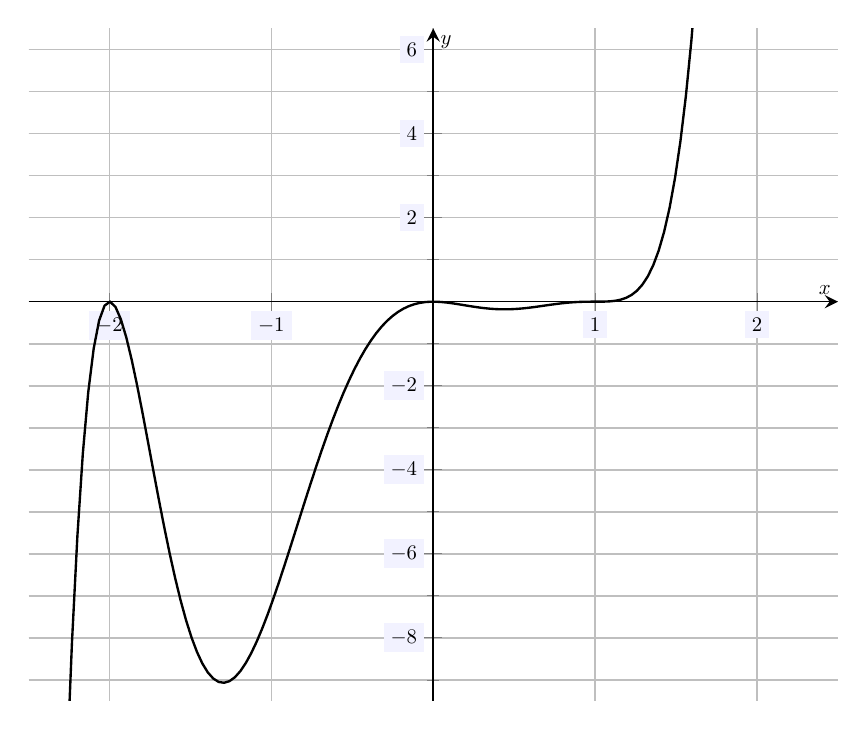
\begin{tikzpicture}[scale=1.5,every node/.style={scale=0.5}]
	\begin{axis}[
	grid=both,
	axis lines=middle,
	ticklabel style={fill=blue!5!white},
	xmin= -2.5, xmax=2.5,
	ymin= -9.5, ymax=6.5,
	xtick={-5,-4,...,5},
	ytick={-10,-8,...,10},
	minor tick = {-10,-9,...,10},
	xlabel=\(x\),ylabel=\(y\),
	]
	\addplot[line width= 0.02cm,samples=150,domain= -2.5:2.5] ({x},{0.9*x^2*(x + 2)^2*(x - 1)^3});
	\end{axis}
	\end{tikzpicture}
	}
	\] \pspace

\sol From the graph of $f(x)$, we can see that $x= -2$, $x= 0$, and $x= 1$ are the only real roots of $f(x)$. 


Furthermore, because the zero at $x= -2$ and $x= 0$ intersects the $x$-axis `tangentially' (not crossing the $x$-axis), the multiplicity of $x= -2$ and $x= 0$ must be at least 2 and must be even. Because the root at $x= 1$ `crosses' the $x$-axis, the multiplicity of $x= 1$ must be at least 1 and must be odd. But then $f(x)$ must have degree at least $2 + 2 + 1= 5$. Because $f(x)$ is a quintic, it has degree 5. Therefore, $f(x)$ cannot have any complex roots. So we know $f(x)$ has the form\dots
	\[
	f(x)= A \big(x - (-2) \big)^2 (x - 0)^2 (x - 1)= A(x + 2)^2 x^2 (x - 1)= A x^2 (x - 1) (x + 2)^2
	\]
We can see that $(-1, -7)$ is a point on the graph of $f(x)$; that is, $f(-1)= -7$. But then\dots
	\[
	\begin{gathered}
	f(x)= A x^2 (x - 1) (x + 2)^2 \\[0.3cm]
	f(-1)= A (-1)^2 (-1 - 1) (-1 + 2)^2 \\[0.3cm]
	-7= -2A \\[0.3cm]
	A= \dfrac{7}{2}
	\end{gathered}
	\]
Therefore, we must have\dots
	\[
	f(x)= \frac{7}{2}\, x^2 (x - 1) (x + 2)^2
	\]


\end{document}